\renewcommand{\thechapter}{\Roman{chapter}}
\chapter{Result and Discussion}
\renewcommand{\thechapter}{\arabic{chapter}}
\label{ch:Result and Discussion}
\thispagestyle{empty}

The results of the system development outlined in the previous chapter were presented and discussed in this chapter. After evaluating the specification of each system and undergo different design revision and integration, the study successfully identified and finalized the necessary components, tools and materials for each system.

\section{Developed 3D Point Cloud Scanner System (3D-PCSS)}

\subsection{3D-PCSS CAD Design Setup}

The 3D Point Cloud Scanner System hardware setup, as shown in Figure \ref{ch4:fig:cad_storage_bin}, consists of a 2D LiDAR Device fixed to a platform connected to a servo motor. This servo motor allows the platform to rotate, giving the LiDAR device an extra axis of movement. Inside the compartment is where the single-board computer along with other circuit components located. The detailed specification of each of the components is presented in appendix \ref{appen:a}.

\begin{figure}[H]
	\centering
	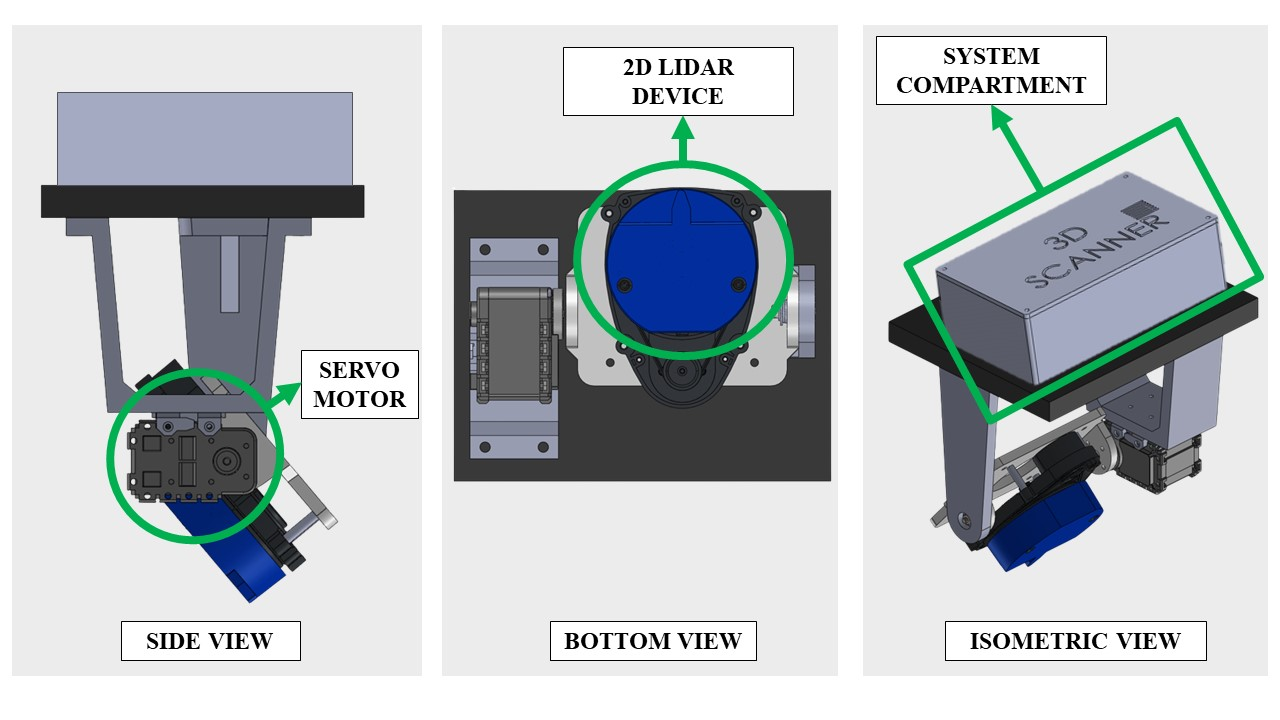
\includegraphics[width=1\textwidth]{Figures/3d-pcss-cad-design}
	\caption{Different View of the CAD Model Design of 3D-PCSS}
	\label{ch4:fig:cad_storage_bin}
\end{figure}

\subsection{Actual Design of the 3D-PCSS}

The actual development of the 3D-PCSS shown in figure \ref{ch4:fig:actual-3d-pcss} was constructed in accordance with the 3D CAD model design and the system is powered by a battery. The base platform, to which the 2D LiDAR device and servo motor are attached, was fabricated using aluminum metal. The system compartment is fabricated using a 3D printer and employing ABS material. Inside the compartment, the specific components and its category is shown in figure \ref{ch4:fig:specific-components}
\begin{figure}[H]
	\centering
	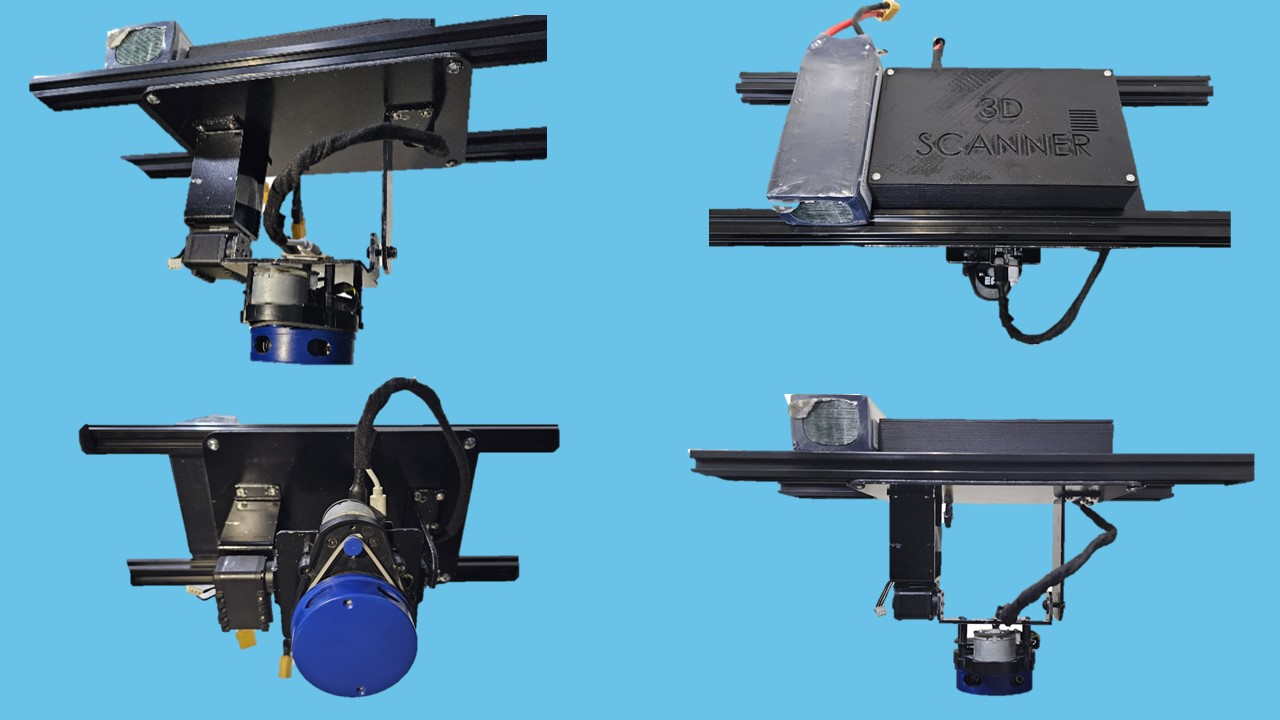
\includegraphics[width=1\textwidth]{Figures/actual-3d-pcss}
	\caption{Actual 3D-PCSS Developed}
	\label{ch4:fig:actual-3d-pcss}
\end{figure}

\begin{figure}[H]
	\centering
	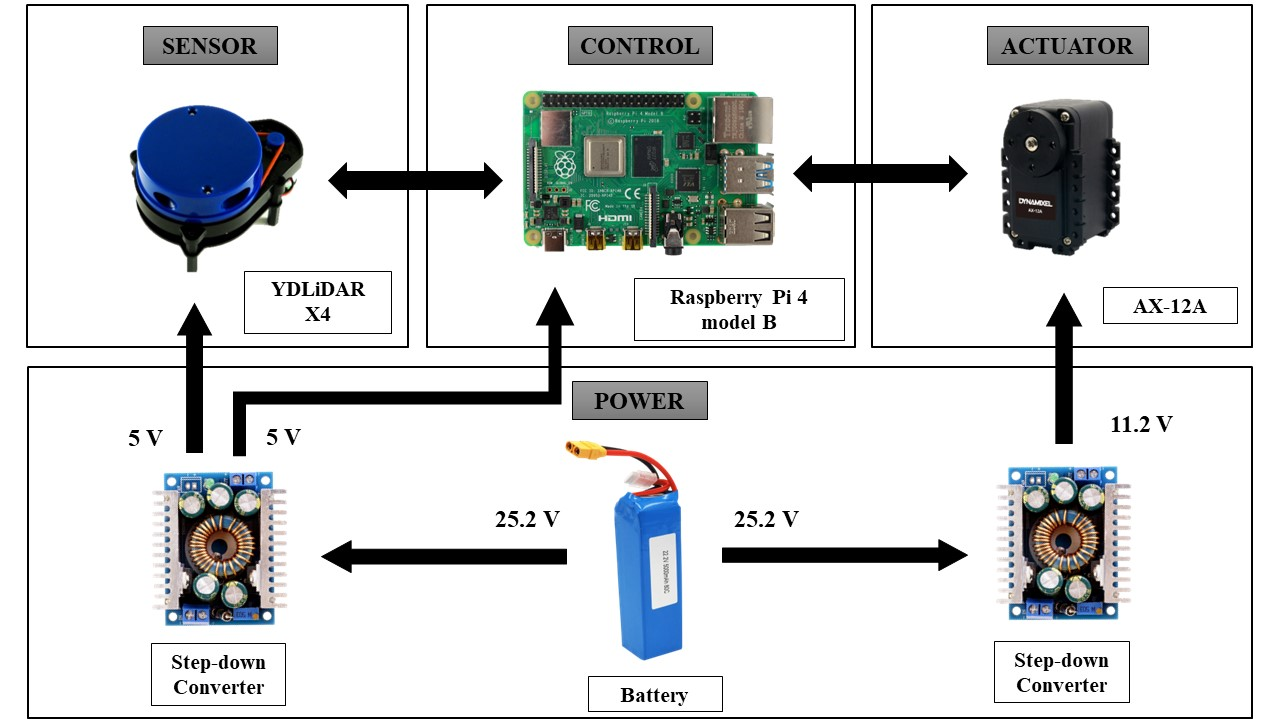
\includegraphics[width=1\textwidth]{Figures/specific-components}
	\caption{Specific Components of the System}
	\label{ch4:fig:specific-components}
\end{figure}

\section{Software Implementation}

The processes discussed in the previous chapter were implemented on the single-board computer (Raspberry Pi), playing a crucial role in the overall functionality of the 3D-PCSS. Figure \ref{ch4:fig:nodes-topics-relationships} illustrates the various nodes, topics, and their relationships in a publish-subscribe model. The arrows in the diagram show how data flows between the different nodes and its relationship to a corresponding topics. The ROS bridge server Node facilitates communication by relaying commands between the web application and the ROS framework via the ``/rosapi" service. Commands to start and stop scanning from the web interface are processed using the Remote Command Node within the system. The LiDAR Node captures data and publishes it as range values, while the Dynamixel Node and LiDAR Node synchronize their operations through the ``/dxl\_pos" topic. The Scan to 3D Point Cloud Mapping Node converts raw scan data into usable 3D point cloud data. Finally, the post-processing stage refines the point cloud data for volume measurement.

\begin{figure}[H]
	\centering
	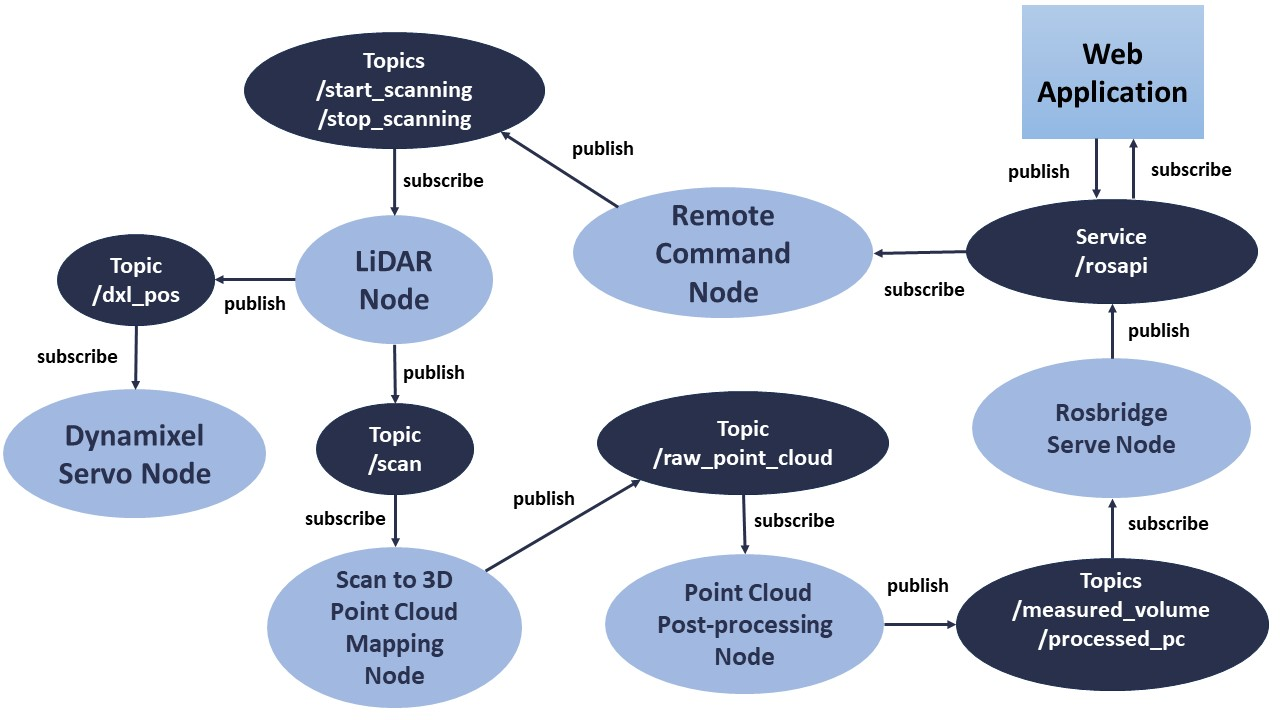
\includegraphics[width=1\textwidth]{Figures/nodes-topics-relationship}
	\caption{Try}
	\label{ch4:fig:nodes-topics-relationships}
\end{figure}

\section{Web-based User Interface Implementation}
A variety set of tools and frameworks were employed to enhance the functionality of the Web Interface. Table \ref{ch3:tab:tools-frameworks} outlines the various tools, frameworks, and libraries utilized in the implementation of the web-based user interface.

\begin{table}[H]
	\centering
	\caption{Tools and Frameworks Used in the Web-based User Interface}
	\label{ch3:tab:tools-frameworks}
	\begin{tabular}{|l|p{9cm}|}
		\hline
		\textbf{Tool/Framework} & \textbf{Description/Functionality}                                                                                                                                                \\ \hline
		jQuery                  & Used for simplifying JavaScript programming and DOM manipulation, jQuery is included via CDN for easy integration.                                                                \\ \hline
		Three.js                & This JavaScript library is utilized for rendering 3D graphics in a web browser. It enables the display of the 3D point cloud viewer within the application.                       \\ \hline
		EventEmitter2           & EventEmitter2 is employed for implementing event-driven programming, allowing efficient communication between different components of the application.                            \\ \hline
		roslib.js               & roslib.js is utilized for connecting the web application to the Robot Operating System (ROS), enabling communication with ROS nodes and topics.                                   \\ \hline
		Bootstrap               & The Bootstrap framework is employed for responsive design and styling of the user interface components. It ensures consistency and enhances the visual appeal of the application. \\ \hline
		Chart.js                & This JavaScript library is used for creating interactive charts and graphs to visualize data. It enhances the user experience by providing intuitive data representation.         \\ \hline
		ros3d.js                & ros3d.js is utilized for integrating ROS visualization capabilities into the web application. It facilitates the display of ROS topics such as point clouds and robot models.     \\ \hline
	\end{tabular}
\end{table}


These tools and frameworks collectively contribute to the functionality of the web-based user interface for the 3D-PCSS.